\documentclass[12pt]{article}
\usepackage{fullpage}
\usepackage{times}
\usepackage{float}
\usepackage[normalem]{ulem}
\usepackage{fancyhdr,graphicx,amsmath,amssymb, mathtools, scrextend, titlesec, enumitem}
\usepackage[ruled,vlined]{algorithm2e} 
\include{pythonlisting}
\usepackage{caption}
\usepackage{subcaption}

\title{Recurrent Neural Networks}
\author{Tadeu Silva (Deds)}
\begin{document}
\maketitle

\begin{figure}[H]
    \centering
    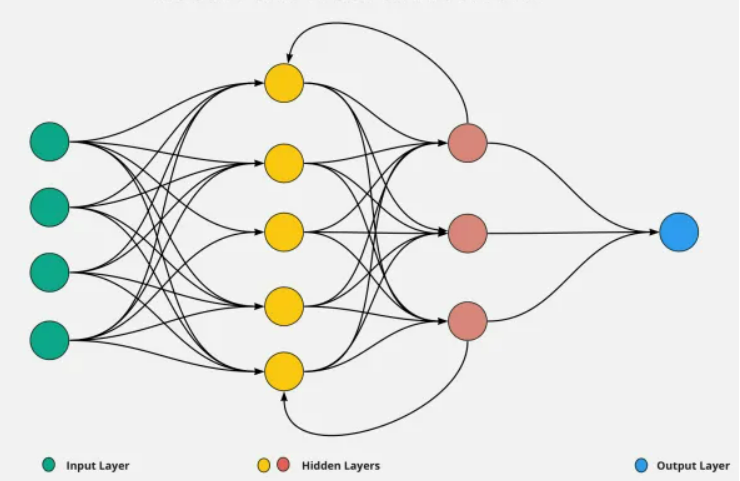
\includegraphics[width=0.9\linewidth]{images/rnn_overview.png}
    \caption{Neural Network Unfolding Source: dataaspirant}
    \label{fig1}
\end{figure}   

\newpage

\section{Introduction}
A Recurrent Neural Network is a type of architecture of Deep Learning which introduces the concept of \textbf{cell state} of a neuron. This allows for handling of sequential/temporal data (like blocs of text). This allows different configurations for training/testing data, as follows:


\begin{figure}[H]
    \centering
    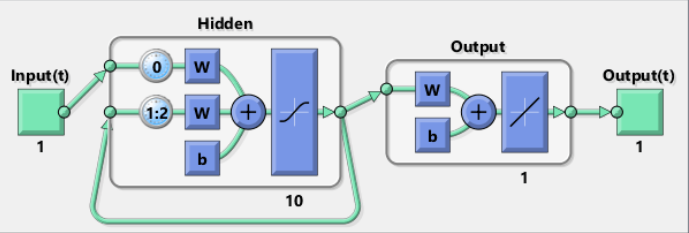
\includegraphics[width=0.79\linewidth]{images/rnn_example.png}
    \caption{Architecture of Recurrent Neural Network}
    \label{fig2}
\end{figure}   


\subsection{Options for Input/Output}
RNN's are very useful because they provide \textbf{memory} for last hidden state, allowing the neurons to remember past configurations. Those elements are really important when handling highly temporal-sensitive data, like understanding a sentence. \mbox{}
\\\\
For example the sentence \textbf{The food was good, not bad at all} vs \textbf{The food was bad, not good at all} shows the importante of order in text. Another important feature is correlation with long periods, like for example the sentence \textbf{Bob is eating an apple. Lisa likes orange. Lisa is having lunch with Bob and she is drinking water.} has various states depending of what the question is asked. So we could ask \textit{who is eating an Apple?} or \textit{Who is drinking water?} and while the latter is easier to answer because the answer is at the end of the phrase, the former is not because we have to propagate the understanding of what Bob is doing throughout the hole sequence of data.
\\\\
This kind of flexibility is reflected on different ways of data handling, like:


\begin{figure}[H]

    \begin{subfigure}[t]{0.3\linewidth}
    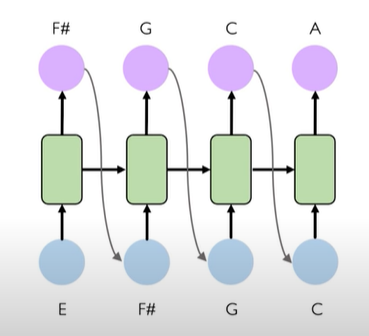
\includegraphics[width=4cm, height=4cm]{images/many_to_many.png}
    \caption{Many to Many}
        
    \end{subfigure}
    \begin{subfigure}[t]{0.3\linewidth}
    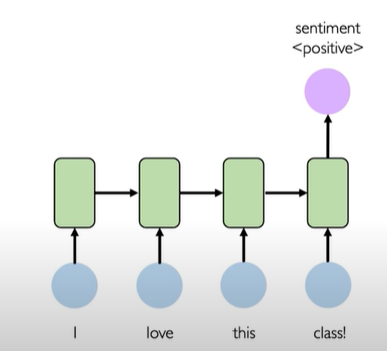
\includegraphics[width=4cm, height=4cm]{images/many_to_one.png}
    \caption{Many to One}

    \end{subfigure}
    \begin{subfigure}[t]{0.3\linewidth}
    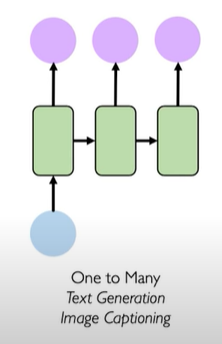
\includegraphics[width=4cm, height=4cm]{images/one_to_many.png}
    \caption{One to Many}

    \end{subfigure}
    \caption{Different ways of Input/Output}
\end{figure}
\mbox{} \\
\textbf{Source of images:} MIT 6.S191: Recurrent Neural Networks - Ava Soleimany

\begin{itemize}
    \item \textbf{Many to Many:} Prediction of the next note for compose music
    \item \textbf{Many to One:} Prediction of sentiment based on given text
    \item \textbf{One to Many:} Generating Text for given Image (number of persons on picture, etc)

\end{itemize}


\section{Forward Pass}

Given an input $\overrightarrow{x}_{t}$ in the Input Layer, the Hidden Layer has output:
\begin{equation}
    a^{1}_{t} = \sigma (z^{1}_{t}) = \sigma({}^{XH}W^{1} \cdot \overrightarrow{x_{t}} + {}^{HH}W \cdot {a^{1}_{t-1}} +  b^{1})
    \label{forward}
\end{equation}
where ${}^{XH}W$ is the \textbf{Input-Hidden Weight} Matrix, ${}^{HH}W$ is the \textbf{Hidden-Hidden Weight} Matrix, $b$ is the \textbf{bias} vector and $\overrightarrow{x_{t}}$ is the \textbf{input} vector.
\\ 
Obs:
\begin{itemize}
    \item $\overrightarrow{x_{t}}$ is a $(m,1)$ vector
    \item ${}^{XH}W$ is a $(n,m)$ matrix
    \item ${}^{HH}W$ is a $(n,n)$ matrix
    \item $b$ is a $(n,1)$ matrix
\end{itemize}

Notice that the difference here is that we take samples of $\overrightarrow{x}$ throughout time. So if we're taking a NLP approach, we may have:

\begin{equation}
    x = ['I', 'love', 'deep', 'learning']
\end{equation}

where:
\begin{itemize}
    \item $x[0] = 'I'$
    \item $x[1] = 'love'$
    \item $x[2] = 'learning'$
    \item $x[3] = 'deep'$
\end{itemize}

and we're taking samples of size $T=4$. So we would repeat equation (\ref{forward}) for every entry of $\overrightarrow{x}$, where we are repetidly updating the 'cell state' of the neuron through time, making sure that the whole phrase is taking in consideration. Of course that when implementing we would change the strings to numbers, via hot-encoding algorithm or word embedding (for not causing too sparse and large binary vectors).


\begin{figure}[H]
    \centering
    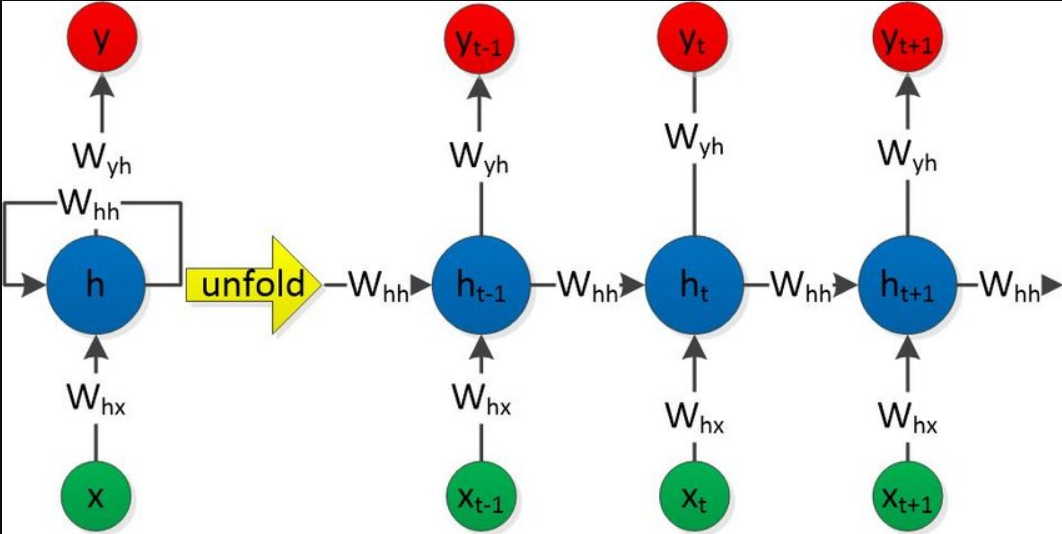
\includegraphics[width=0.7\linewidth]{images/rnn_unfolding.png}
    \caption{Acumulation through time in a RNN. $W_{hh}, W_{hx}, W_{yh}$ fixed in time. Source: researchgate }
    \label{fig2}
\end{figure}   


\subsection{Example}

In a simple 2-3-2 Layer Type of Network, we have:


\begin{figure}[H]
    \centering
    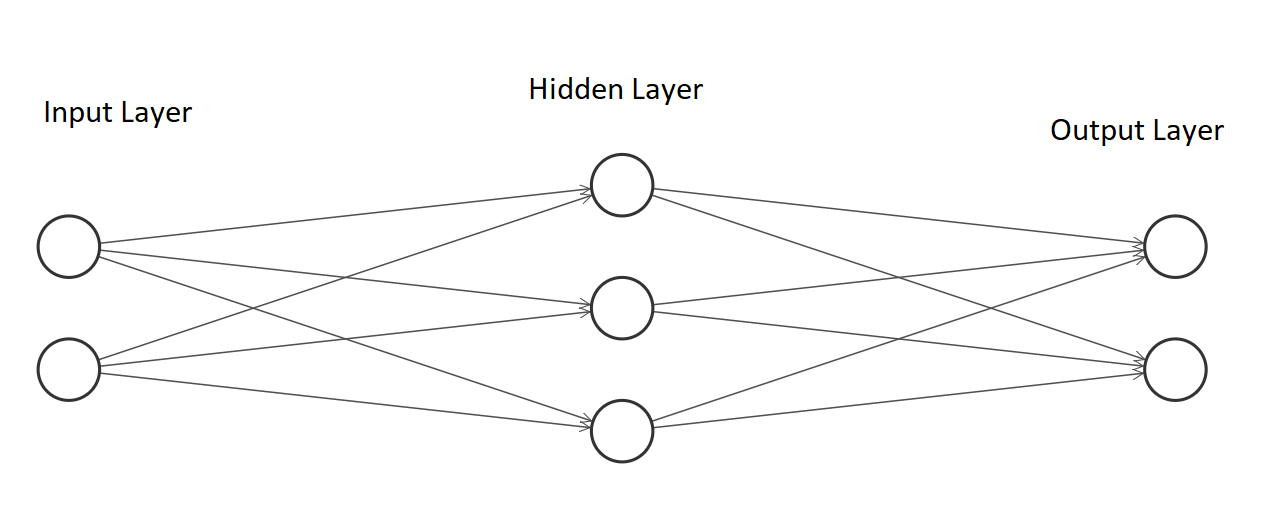
\includegraphics[width=0.7\linewidth]{images/example.png}
    \caption{Simple 2-3-2 Recurrent Neural Network Example}
\end{figure}   

\textbf{Input Layer - Hidden Layer}
\begin{equation}
\begin{bmatrix}
a_{1}^{1}\\
a_{2}^{1}\\
a_{3}^{1}
\end{bmatrix}_{t}
=
\sigma
\left(
\begin{bmatrix}
x_{1}\\
x_{2}
\end{bmatrix}_{t}
\cdot
\begin{bmatrix}
{}^{hx}W_{11} & {}^{hx}W_{12}\\
{}^{hx}W_{21} & {}^{hx}W_{22}\\
{}^{hx}W_{31} & {}^{hx}W_{32}
\end{bmatrix}
 +
\begin{bmatrix}
a_{1}^{1}\\
a_{2}^{1}\\
a_{3}^{1}
\end{bmatrix}_{t-1}
\cdot
\begin{bmatrix}
{}^{hh}W_{11} & {}^{hh}W_{12} & {}^{hh}W_{13}\\
{}^{hh}W_{21} & {}^{hh}W_{22} & {}^{hh}W_{23}\\
{}^{hh}W_{31} & {}^{hh}W_{32} & {}^{hh}W_{33}\\
\end{bmatrix}
 +
 \begin{bmatrix}
b_{1}^{1}\\
b_{2}^{1}\\
b_{3}^{1}
\end{bmatrix}
\right)
\end{equation}
\\

\textbf{Hidden Layer - Output Layer}
\begin{equation}
\begin{bmatrix}
a_{1}^{2}\\
a_{2}^{2}
\end{bmatrix}_{t}
=
\sigma
\left(
\begin{bmatrix}
z_{1}^{2}\\
z_{2}^{2}
\end{bmatrix}_{t}
\right)
=
\sigma
\left(
\begin{bmatrix}
a_{1}^{1}\\
a_{2}^{1}\\
a_{3}^{1}
\end{bmatrix}_{t}
\cdot
\begin{bmatrix}
{}^{hy}W_{11} & {}^{hy}W_{12} & {}^{hy}W_{13} \\
{}^{hy}W_{21} & {}^{hy}W_{22} & {}^{hy}W_{23} \\ 
\end{bmatrix}
 +
 \begin{bmatrix}
b_{1}^{2}\\
b_{2}^{2}
\end{bmatrix}
\right)
\end{equation}

\section{Backward Pass}
\subsection{Loss}
In the Backward pass, we first compute our \textbf{loss} (aka the error of our output) and average along the data, to get a measure of our total uncertainty. The difference on the RNNs is that we need to compute all the gradients from previous timesteps. We have:
\begin{equation}
    loss = (\dfrac{1}{n}) \sum_{i=0}^{n} \mu \left( loss(a_{i,t}^{2}, y_{i,t}) \right) = (\dfrac{1}{T}) (\dfrac{1}{n}) \sum_{i=0}^{n} \sum_{t=0}^{T} \mu \left( loss(a_{i,t}^{2}, y_{i,t}) \right)
\end{equation}
Where $\mu$ is the temporal average on the column matrix. So for our example:
\begin{equation}
    loss = (\dfrac{1}{T}) (\dfrac{1}{2}) \sum_{t=0}^{T} \mu \left(
\begin{bmatrix}
(a_{1}^{2} - y_{1})^2\\
(a_{2}^{2} - y_{2})^2\\
\end{bmatrix}_{t}
\right) =
(\dfrac{1}{T}) (\dfrac{1}{2}) \sum_{t=0}^{T} \left(
(a_{1}^{2} - y_{1})^2 + (a_{2}^{2} - y_{2})^2
\right) _{t}
\end{equation}
where n is the dimension of the output layer, using the \textbf{Mean Squared Error} (which is not recommendable for probability distribution problems, like NLP.

\subsection{Backpropagation Through Time (BTT)}
The second part is to calculate how each weight and bias had influence in the loss, for every timestep taken. So we want to calculate:
\begin{equation}
\nabla C
=
\begin{bmatrix}
\dfrac{\partial C}{\partial W} \\\\
\dfrac{\partial C}{\partial b} 
\end{bmatrix},
\dfrac{\partial C}{\partial W} = 
\begin{bmatrix}
\dfrac{\partial C}{\partial {}^{hx}W} \\\\
\dfrac{\partial C}{\partial {}^{hh}W} \\\\
\dfrac{\partial C}{\partial {}^{hy}W} \\\\
\end{bmatrix},
\dfrac{\partial C}{\partial W} = 
\begin{bmatrix}
\dfrac{\partial C}{\partial b_{1}} \\\\
\dfrac{\partial C}{\partial b_{2}} 
\end{bmatrix}
\end{equation}
We do that using the Backpropagation (chain rule). Remembering from calculus, the derivative of a composite function $f(g(x))$ can be written as:
\begin{equation}
    \dfrac{df}{dx} = \dfrac{df}{dg} \dfrac{dg}{dx}
\end{equation}

So applying these concepts for the layers, we have:

\begin{equation}
    \dfrac{\partial C}{\partial W} = \left( \dfrac{\partial C}{\partial a}\right) \left( \dfrac{\partial a}{\partial z}\right) \left(\dfrac{\partial z}{\partial W} \right)
\end{equation}
\begin{equation}
    \dfrac{\partial C}{\partial b} = \left( \dfrac{\partial C}{\partial a}\right) \left( \dfrac{\partial a}{\partial z}\right) \left(\dfrac{\partial z}{\partial b} \right)
\end{equation} \mbox{} \\

The activation function $\sigma$ depends on the problem at hand. But let's suppose we are at a \textbf{classification} problem, so we'll go with the \textbf{Softmax} function, defined as:

\begin{equation}
    \sigma (z) = \dfrac{e^{z}}{\sum_{j=0}^{n} e^{z_{j}}}
\end{equation}

So the derivative is:

\[
\dfrac{d \sigma}{\partial z} = z ( 1 - z )
\] \mbox{} \\

Let's denote the following two operations:
\begin{itemize}
    \item $\times$ : element-wise multiplication, i.e. same dimensions only
    \item $\cdot$ : dot product, i.e (m,k) $\cdot$ (k,n) = (m,n)
\end{itemize}

This means that if:
\[
A =
\begin{bmatrix}
a_{11} & a_{12}\\
a_{21} & a_{22}
\end{bmatrix}
, B = 
\begin{bmatrix}
b_{11} & b_{12}\\
b_{21} & b_{22}
\end{bmatrix}
\Rightarrow
A X B = 
\begin{bmatrix}
a_{11}\cdot b_{11} & a_{12}\cdot b_{12}\\
a_{21}\cdot b_{21} & a_{22}\cdot b_{22}
\end{bmatrix}
\] 

Analogously, if:
\[
A =
\begin{bmatrix}
a_{11} & a_{12}\\
a_{21} & a_{22}
\end{bmatrix}
, B = 
\begin{bmatrix}
b_{11}\\
b_{21}
\end{bmatrix}
\Rightarrow
A \cdot B = 
\begin{bmatrix}
a_{11}\cdot b_{11} + a_{12}\cdot b_{21}\\
a_{21}\cdot b_{11} + a_{22}\cdot b_{21}
\end{bmatrix}
\] 



Analyzing the nuances for each layer, we have:

\paragraph{1. Output - Hidden Layer} \mbox{} \\
For the Output Layer, we get:

\begin{equation}
    \dfrac{\partial C}{\partial {}^{hy}W} = \left( \dfrac{\partial C}{\partial a^{2}}\right) \left( \dfrac{\partial a^{2}}{\partial z^{2}}\right) \left(\dfrac{\partial z^{2}}{\partial {}^{hy}W} \right)
\end{equation}

\[
\dfrac{\partial C}{\partial a^{2}} =  (\dfrac{1}{T}) \sum_{t=0}^{T} 2(a_{2}^{2} - y_{i})_{t} = (\dfrac{2}{T}) \sum_{t=0}^{T} 
\begin{bmatrix}
(a_{1}^{2} - y_{1})\\
(a_{2}^{2} - y_{2})\\
\end{bmatrix}_{t}
\]

\[
\dfrac{\partial a^{2}}{\partial z^{2}} = \dfrac{d \sigma}{\partial z^{2}} = (\dfrac{1}{T}) \sum_{t=0}^{T} z^{2}_{t} ( 1 - z^{2} )_{t} = (\dfrac{1}{T}) \sum_{t=0}^{T} 
\begin{bmatrix}
z_{1}^{2}(1 - z_{1}^{2})\\
z_{2}^{2}(1 - z_{2}^{2})\\
\end{bmatrix}_{t}
\]

\[
\dfrac{\partial z^{2}}{\partial {}^{hy}W} = (\dfrac{1}{T}) \sum_{t=0}^{T} a^{1}_{t} = (\dfrac{1}{T}) \sum_{t=0}^{T} 
\begin{bmatrix}
a_{1}^{1}\\
a_{2}^{1}\\
a_{3}^{1}
\end{bmatrix}_{t}
\]

So we have:

\[
\dfrac{\partial C}{\partial {}^{hy}W} 
=
(\dfrac{1}{T}) \sum_{t=0}^{T} 
\Bigg[
\begin{bmatrix}
2(a_{1}^{2} - y_{1})\\
2(a_{2}^{2} - y_{2})\\
\end{bmatrix}_{t}
\times
\begin{bmatrix}
z_{1}^{2}(1 - z_{1}^{2})\\
z_{2}^{2}(1 - z_{2}^{2})\\
\end{bmatrix}_{t}
\cdot
\left(
\begin{bmatrix}
a_{1}^{1}\\
a_{2}^{1}\\
a_{3}^{1}
\end{bmatrix}_{t}
\right)^{T}
\Bigg]
\]

Analogously, for the bias:

\begin{equation}
    \dfrac{\partial C}{\partial b^{2}} = \left( \dfrac{\partial C}{\partial a^{2}}\right) \left( \dfrac{\partial a^{2}}{\partial z^{2}}\right) \left(\dfrac{\partial z^{2}}{\partial b^{2}} \right)
\end{equation}

So the two terms are the same. For the last one, note that because of the definition of $z^{2}$:

\[
\dfrac{\partial z^{2}}{\partial b^{2}} = 1
\]

Then we get:


\[
\dfrac{\partial C}{\partial a^{2}} 
=
(\dfrac{1}{T}) \sum_{t=0}^{T} 
\Bigg[
\begin{bmatrix}
2(a_{1}^{2} - y_{1})\\
2(a_{2}^{2} - y_{2})\\
\end{bmatrix}_{t}
\times
\begin{bmatrix}
z_{1}^{2}(1 - z_{1}^{2})\\
z_{2}^{2}(1 - z_{2}^{2})\\
\end{bmatrix}_{t}
\Bigg]
\]


\paragraph{1. Hidden - Input Layer} \mbox{} \\

Analogously we have:

\begin{equation}
    \dfrac{\partial C}{\partial {}^{hx}W} = \left( \dfrac{\partial C}{\partial a^{1}}\right) \left( \dfrac{\partial a^{1}}{\partial z^{1}}\right) \left(\dfrac{\partial z^{1}}{\partial {}^{hx}W} \right)
    \label{whx}
\end{equation}

\[
\dfrac{\partial C}{\partial a^{1}}
=
\left(\dfrac{\partial C}{\partial a^{2}}\right)
\left(\dfrac{\partial a^{2}}{\partial z^{2}}\right)
\left(\dfrac{\partial z^{2}}{\partial a^{1}}\right)
\]

Note that, by definition:

\[
\dfrac{\partial z^{2}}{\partial a^{1}} = {}^{hy}W
\]

So:

\[
\dfrac{\partial C}{\partial a^{1}}
=
\left(
(\dfrac{1}{T}) \sum_{t=0}^{T} 
\Bigg[
\begin{bmatrix}
2(a_{1}^{2} - y_{1})\\
2(a_{2}^{2} - y_{2})\\
\end{bmatrix}_{t}
\times
\begin{bmatrix}
z_{1}^{2}(1 - z_{1}^{2})\\
z_{2}^{2}(1 - z_{2}^{2})\\
\end{bmatrix}_{t}
\Bigg]^{T}
\cdot
\begin{bmatrix}
{}^{hy}W_{11} & {}^{hy}W_{12} & {}^{hy}W_{13} \\
{}^{hy}W_{21} & {}^{hy}W_{22} & {}^{hy}W_{23} \\ 
\end{bmatrix}
\right)^{T}
\]

The second term from equation (\ref{whx}) is:

\[
\dfrac{\partial a^{1}}{\partial z^{1}}
=
\begin{bmatrix}
z_{1}^{1}(1 - z_{1}^{1})\\
z_{2}^{1}(1 - z_{2}^{1})\\
z_{3}^{1}(1 - z_{3}^{1})
\end{bmatrix}_{t}
\]

For the last term, let's check what happens with t=0:

\[
z^{1}_{0}
=
x_{0} \cdot {}^{hx}W + b^{1}
\Rightarrow
\dfrac{\partial z^{1}_{0}}{\partial {}^{hx}W}
=
x_{0}
\]

Now for t = 1:

\[
z^{1}_{1}
=
x_{1} \cdot {}^{hx}W + a^{1}_{0} \cdot {}^{hh}W +  b^{1}
=
x_{1} \cdot {}^{hx}W + \sigma(z^{1}_{0}) \cdot {}^{hh}W +  b^{1}
\]
\[
\Rightarrow
\dfrac{\partial z^{1}_{1}}{\partial {}^{hx}W}
=
x_{1} + z^{1}_{0} (1 - z^{1}_{0})x_{0} \cdot {}^{hh}W
\]

If we do it one more time, for t = 2, we can see the pattern happening:


\[
z^{1}_{2}
=
x_{2} \cdot {}^{hx}W + a^{1}_{1} \cdot {}^{hh}W +  b^{1}
=
x_{2} \cdot {}^{hx}W + \sigma(z^{1}_{1}) \cdot {}^{hh}W +  b^{1}
\]
\[
\Rightarrow
\dfrac{\partial z^{1}_{2}}{\partial {}^{hx}W}
=
x_{2} + z^{1}_{1} (1 - z^{1}_{1})\big[ x_{1} + z^{1}_{0} (1 - z^{1}_{0})x_{0} \cdot {}^{hh}W\big] \cdot {}^{hh}W
\]

So we are acumulating the derivatives of past timesteps. Reorganizing the terms, we can rewrite the above equations as:

\[
t = 0: 
\dfrac{\partial z^{1}_{0}}{\partial {}^{hx}W} = x_{0}
\]
\[
t = 1:
\dfrac{\partial z^{1}_{1}}{\partial {}^{hx}W}
=
x_{1} + \sigma^{'}(z^{1}_{0}) \Big (\dfrac{\partial z^{1}_{0}}{\partial {}^{hx}W} \Big )\cdot {}^{hh}W
\]
\[
t = 2:
\dfrac{\partial z^{1}_{2}}{\partial {}^{hx}W}
=
x_{2} + \sigma^{'}(z^{1}_{1}) \Big (\dfrac{\partial z^{1}_{1}}{\partial {}^{hx}W} \Big )\cdot {}^{hh}W
\]
\[
t = k:
\dfrac{\partial z^{1}_{k}}{\partial {}^{hx}W}
=
x_{k} + \sigma^{'}(z^{1}_{k-1}) \Big (\dfrac{\partial z^{1}_{k-1}}{\partial {}^{hx}W} \Big )\cdot {}^{hh}W
\]

Congratulations! If you understood the above derivation, you now understands the \textbf{Backpropagation Through Time}, the most complex of the backpropagation family for Deep Learning.

\mbox{} \\\\
Wrapping things up, from equation (\ref{whx}) we have:

    
\[
\dfrac{\partial C}{\partial {}^{hx}W}
=
(\dfrac{1}{T}) \sum_{t=0}^{T} 
\Bigg(
\left( \dfrac{\partial C}{\partial a_{2}}\right)
\times 
\begin{bmatrix}
z_{1}^{1}(1 - z_{1}^{1})\\
z_{2}^{1}(1 - z_{2}^{1})\\
z_{3}^{1}(1 - z_{3}^{1})
\end{bmatrix}_{t}
\cdot
\Big (
x_{t} + \sigma^{'}(z^{1}_{t-1}) \Big (\dfrac{\partial z^{1}_{t-1}}{\partial {}^{hx}W} \Big )\cdot {}^{hh}W
\Big )^{T}
\Bigg)
\]

The good news is that the other derivative for the weight ${}^{hh}W$ is very similar to the previous one. So this will be a good reminder that you understood the equations. Let's dive in:

\mbox{} \\

Generally we have:

\begin{equation}
    \dfrac{\partial C}{\partial {}^{hh}W} = \left( \dfrac{\partial C}{\partial a^{1}}\right) \left( \dfrac{\partial a^{1}}{\partial z^{1}}\right) \left(\dfrac{\partial z^{1}}{\partial {}^{hh}W} \right)
    \label{whh}
\end{equation}

The first two terms are the same as above, there is: 


\[
\dfrac{\partial C}{\partial a^{1}}
=
\left(
(\dfrac{1}{T}) \sum_{t=0}^{T} 
\Bigg[
\begin{bmatrix}
2(a_{1}^{2} - y_{1})\\
2(a_{2}^{2} - y_{2})\\
\end{bmatrix}_{t}
\times
\begin{bmatrix}
z_{1}^{2}(1 - z_{1}^{2})\\
z_{2}^{2}(1 - z_{2}^{2})\\
\end{bmatrix}_{t}
\Bigg]^{T}
\cdot
\begin{bmatrix}
{}^{hy}W_{11} & {}^{hy}W_{12} & {}^{hy}W_{13} \\
{}^{hy}W_{21} & {}^{hy}W_{22} & {}^{hy}W_{23} \\ 
\end{bmatrix}
\right)^{T}
\]

And:

\[
\dfrac{\partial a^{1}}{\partial z^{1}}
=
\begin{bmatrix}
z_{1}^{1}(1 - z_{1}^{1})\\
z_{2}^{1}(1 - z_{2}^{1})\\
z_{3}^{1}(1 - z_{3}^{1})
\end{bmatrix}_{t}
\]

The last term is the one we need to be careful, due the time dependence. So let's do the same analysis. For t = 0 we have:

\[
z^{1}_{0}
=
x_{0} \cdot {}^{hx}W + b^{1}
\Rightarrow
\dfrac{\partial z^{1}_{0}}{\partial {}^{hh}W} = 0
\]

Now, for t = 1 we have:


\[
z^{1}_{1}
=
x_{1} \cdot {}^{hx}W + a^{1}_{0} \cdot {}^{hh}W +  b^{1}
\Rightarrow
\dfrac{\partial z^{1}_{1}}{\partial {}^{hh}W} 
=
a^{1}_{0}
\]

Finally, for t = 2:

\[
z^{1}_{2}
=
x_{2} \cdot {}^{hx}W + a^{1}_{1} \cdot {}^{hh}W +  b^{1}
\Rightarrow
\dfrac{\partial z^{1}_{2}}{\partial {}^{hh}W} = a^{1}_{1}
\]

So, for t = k:

\[
z^{1}_{k}
=
x_{k} \cdot {}^{hx}W + a^{1}_{k-1} \cdot {}^{hh}W +  b^{1}
\Rightarrow
\dfrac{\partial z^{1}_{k}}{\partial {}^{hh}W} = a^{1}_{k-1}
\]


Much easier! Summarizing, from equation (\ref{whh}) we then get:


\[
\dfrac{\partial C}{\partial {}^{hh}W}
=
(\dfrac{1}{T}) \sum_{t=0}^{T} 
\Bigg(
\left( \dfrac{\partial C}{\partial a_{2}}\right)
\times 
\begin{bmatrix}
z_{1}^{1}(1 - z_{1}^{1})\\
z_{2}^{1}(1 - z_{2}^{1})\\
z_{3}^{1}(1 - z_{3}^{1})
\end{bmatrix}_{t}
\cdot
\begin{bmatrix}
a_{1}^{1}\\
a_{2}^{1}\\
a_{3}^{1}
\end{bmatrix}_{t-1}
\Bigg)
\]

Finally, for the bias we have:

\begin{equation}
    \dfrac{\partial C}{\partial b^{1}} = \left( \dfrac{\partial C}{\partial a^{1}}\right) \left( \dfrac{\partial a^{1}}{\partial z^{1}}\right) \left(\dfrac{\partial z^{1}}{\partial b^{1}} \right)
\end{equation}

So, the same way as before, by definition:

\[
\dfrac{\partial z^{1}}{\partial b^{1}} = 1
\]

We then have:

\[
    \dfrac{\partial C}{\partial b^{1}} = \left( \dfrac{\partial C}{\partial a^{1}}\right) \left( \dfrac{\partial a^{1}}{\partial z^{1}}\right)
\]

\subsection{Optimizing}
For the last step, we optimize the weights accordingly to the changes calculated on the previous section. There are a few optimizers, but the two most used are: \textbf{SGD} (Stochastic Gradient Descent) and \textbf{Adam}.   \mbox{} \\

\paragraph{SGD - Stochastic Gradient Descent} \mbox{} \\
The SGD is based in the simple idea that: the gradient shows the growth direction. Because we want to \textbf{decrease} our error/loss, we simple get the opposite direction adding the minus sign. So the equation is:

\begin{equation}
    {}^{hy}W = W^{l} - lr \times \dfrac{\partial C}{\partial {}^{hy}W}
\end{equation}
\begin{equation}
    {}^{hx}W = W^{l} - lr \times \dfrac{\partial C}{\partial {}^{hx}W}
\end{equation}
\begin{equation}
    {}^{hh}W = W^{l} - lr \times \dfrac{\partial C}{\partial {}^{hh}W}
\end{equation}
\begin{equation}
    b^{1} = b^{l} - lr \times \dfrac{\partial C}{\partial b^{1}}
\end{equation}
\begin{equation}
    b^{2} = b^{l} - lr \times \dfrac{\partial C}{\partial b^{2}}
\end{equation}
where lr is the \textbf{learning rate}, a parameter $( lr < 1 )$ just to make sure that we don't make great jumps and `miss` the local minima.

\end{document}